\documentclass{scrartcl}
\usepackage{mathtools}
\usepackage{tikz}
\usetikzlibrary{trees,positioning}

\begin{document}
\begin{figure}
\centering
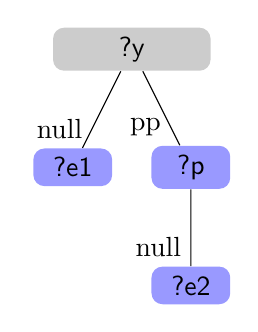
\begin{tikzpicture}
\node[fill = gray!40, shape = rectangle, rounded corners, minimum width = 2cm, font = \sffamily] (70) {?y}
child {node[fill = blue!40, shape = rectangle, rounded corners, minimum width = 1cm, font = \sffamily]  (71) {?e1}
}
child {node[fill = blue!40, shape = rectangle, rounded corners, minimum width = 1cm, font = \sffamily]  (72) {?p}
child {node[fill = blue!40, shape = rectangle, rounded corners, minimum width = 1cm, font = \sffamily] (73) {?e2}
}
};
\begin{scope}[nodes = {draw = none}]
\path (71)     -- (70) node [near start, left]  {\text{null}};
\path (72)     -- (70) node [near start, left]  {\text{pp}};
\path (73)     -- (72) node [near start, left]  {\text{null}};
\draw[densely dashed, rounded corners, thin];
\end{scope} 
\end{tikzpicture}
\caption{Visualisation for SPARQLPattern\_DE\_1}
\label{fig:SPARQLPatternDE1}
\end{figure}


\begin{figure}
\centering
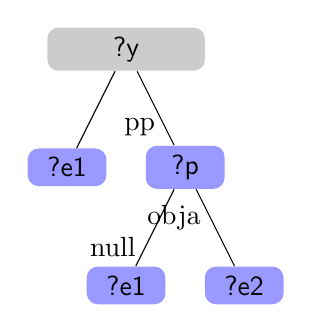
\begin{tikzpicture}
\node[fill = gray!40, shape = rectangle, rounded corners, minimum width = 2cm, font = \sffamily] (73) {?y}
child {node[fill = blue!40, shape = rectangle, rounded corners, minimum width = 1cm, font = \sffamily]  (74) {?e1}
}
child {node[fill = blue!40, shape = rectangle, rounded corners, minimum width = 1cm, font = \sffamily]  (75) {?p}
child {node[fill = blue!40, shape = rectangle, rounded corners, minimum width = 1cm, font = \sffamily] (76) {?e1}
}
child {node[fill = blue!40, shape = rectangle, rounded corners, minimum width = 1cm, font = \sffamily]  (77) {?e2}
}
};
\begin{scope}[nodes = {draw = none}]
\path (76)     -- (75) node [near start, left]  {\text{null}};
\path (75)     -- (73) node [near start, left]  {\text{pp}};
\path (77)     -- (73) node [near start, left]  {\text{obja}};
\draw[densely dashed, rounded corners, thin];
\end{scope} 
\end{tikzpicture}
\caption{Visualisation for SPARQLPattern\_DE\_2}
\label{fig:SPARQLPatternDE2}
\end{figure}


\begin{figure}
\centering
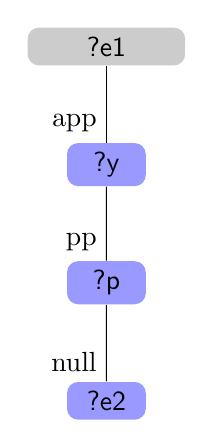
\begin{tikzpicture}
\node[fill = gray!40, shape = rectangle, rounded corners, minimum width = 2cm, font = \sffamily] (77) {?e1}
child {node[fill = blue!40, shape = rectangle, rounded corners, minimum width = 1cm, font = \sffamily]  (78) {?y}
child {node[fill = blue!40, shape = rectangle, rounded corners, minimum width = 1cm, font = \sffamily] (79) {?p}
child {node[fill = blue!40, shape = rectangle, rounded corners, minimum width = 1cm, font = \sffamily] (80) {?e2}
}
}};
\begin{scope}[nodes = {draw = none}]
\path (78)     -- (77) node [near start, left]  {\text{app}};
\path (79)     -- (78) node [near start, left]  {\text{pp}};
\path (80)     -- (79) node [near start, left]  {\text{null}};
\draw[densely dashed, rounded corners, thin];
\end{scope} 
\end{tikzpicture}
\caption{Visualisation for SPARQLPattern\_DE\_3}
\label{fig:SPARQLPatternDE3}
\end{figure}


\begin{figure}
\centering
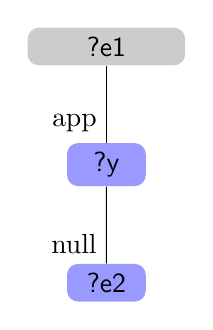
\begin{tikzpicture}
\node[fill = gray!40, shape = rectangle, rounded corners, minimum width = 2cm, font = \sffamily] (80) {?e1}
child {node[fill = blue!40, shape = rectangle, rounded corners, minimum width = 1cm, font = \sffamily]  (81) {?y}
child {node[fill = blue!40, shape = rectangle, rounded corners, minimum width = 1cm, font = \sffamily] (82) {?e2}
}
};
\begin{scope}[nodes = {draw = none}]
\path (81)     -- (80) node [near start, left]  {\text{app}};
\path (82)     -- (81) node [near start, left]  {\text{null}};
\draw[densely dashed, rounded corners, thin];
\end{scope} 
\end{tikzpicture}
\caption{Visualisation for SPARQLPattern\_DE\_4}
\label{fig:SPARQLPatternDE4}
\end{figure}


null


\begin{figure}
\centering
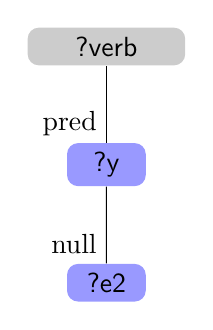
\begin{tikzpicture}
\node[fill = gray!40, shape = rectangle, rounded corners, minimum width = 2cm, font = \sffamily] (82) {?verb}
child {node[fill = blue!40, shape = rectangle, rounded corners, minimum width = 1cm, font = \sffamily]  (83) {?y}
child {node[fill = blue!40, shape = rectangle, rounded corners, minimum width = 1cm, font = \sffamily] (84) {?e2}
}
};
\begin{scope}[nodes = {draw = none}]
\path (83)     -- (82) node [near start, left]  {\text{pred}};
\path (84)     -- (83) node [near start, left]  {\text{null}};
\draw[densely dashed, rounded corners, thin];
\end{scope} 
\end{tikzpicture}
\caption{Visualisation for SPARQLPattern\_DE\_6}
\label{fig:SPARQLPatternDE6}
\end{figure}


\begin{figure}
\centering
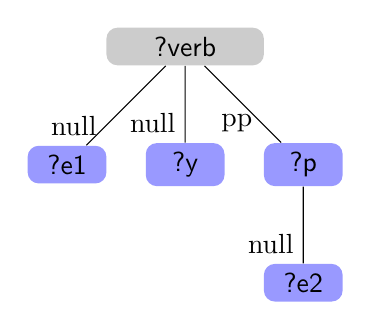
\begin{tikzpicture}
\node[fill = gray!40, shape = rectangle, rounded corners, minimum width = 2cm, font = \sffamily] (84) {?verb}
child {node[fill = blue!40, shape = rectangle, rounded corners, minimum width = 1cm, font = \sffamily]  (85) {?e1}
}
child {node[fill = blue!40, shape = rectangle, rounded corners, minimum width = 1cm, font = \sffamily]  (86) {?y}
}
child {node[fill = blue!40, shape = rectangle, rounded corners, minimum width = 1cm, font = \sffamily]  (87) {?p}
child {node[fill = blue!40, shape = rectangle, rounded corners, minimum width = 1cm, font = \sffamily] (88) {?e2}
}
};
\begin{scope}[nodes = {draw = none}]
\path (85)     -- (84) node [near start, left]  {\text{null}};
\path (86)     -- (84) node [near start, left]  {\text{null}};
\path (87)     -- (84) node [near start, left]  {\text{pp}};
\path (88)     -- (87) node [near start, left]  {\text{null}};
\draw[densely dashed, rounded corners, thin];
\end{scope} 
\end{tikzpicture}
\caption{Visualisation for SPARQLPattern\_DE\_7}
\label{fig:SPARQLPatternDE7}
\end{figure}


\begin{figure}
\centering
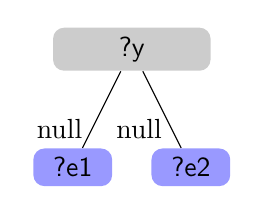
\begin{tikzpicture}
\node[fill = gray!40, shape = rectangle, rounded corners, minimum width = 2cm, font = \sffamily] (88) {?y}
child {node[fill = blue!40, shape = rectangle, rounded corners, minimum width = 1cm, font = \sffamily]  (89) {?e1}
}
child {node[fill = blue!40, shape = rectangle, rounded corners, minimum width = 1cm, font = \sffamily]  (90) {?e2}
}
;
\begin{scope}[nodes = {draw = none}]
\path (89)     -- (88) node [near start, left]  {\text{null}};
\path (90)     -- (88) node [near start, left]  {\text{null}};
\draw[densely dashed, rounded corners, thin];
\end{scope} 
\end{tikzpicture}
\caption{Visualisation for SPARQLPattern\_DE\_8}
\label{fig:SPARQLPatternDE8}
\end{figure}


\begin{figure}
\centering
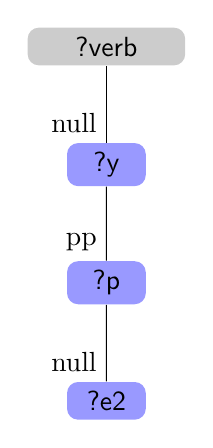
\begin{tikzpicture}
\node[fill = gray!40, shape = rectangle, rounded corners, minimum width = 2cm, font = \sffamily] (90) {?verb}
child {node[fill = blue!40, shape = rectangle, rounded corners, minimum width = 1cm, font = \sffamily]  (91) {?y}
child {node[fill = blue!40, shape = rectangle, rounded corners, minimum width = 1cm, font = \sffamily] (92) {?p}
child {node[fill = blue!40, shape = rectangle, rounded corners, minimum width = 1cm, font = \sffamily] (93) {?e2}
}
}};
\begin{scope}[nodes = {draw = none}]
\path (91)     -- (90) node [near start, left]  {\text{null}};
\path (92)     -- (91) node [near start, left]  {\text{pp}};
\path (93)     -- (92) node [near start, left]  {\text{null}};
\draw[densely dashed, rounded corners, thin];
\end{scope} 
\end{tikzpicture}
\caption{Visualisation for SPARQLPattern\_DE\_9}
\label{fig:SPARQLPatternDE9}
\end{figure}


\begin{figure}
\centering
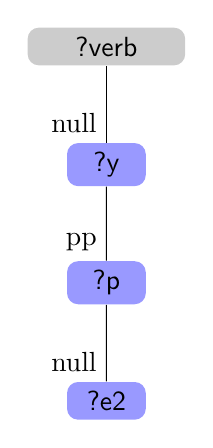
\begin{tikzpicture}
\node[fill = gray!40, shape = rectangle, rounded corners, minimum width = 2cm, font = \sffamily] (93) {?verb}
child {node[fill = blue!40, shape = rectangle, rounded corners, minimum width = 1cm, font = \sffamily]  (94) {?y}
child {node[fill = blue!40, shape = rectangle, rounded corners, minimum width = 1cm, font = \sffamily] (95) {?p}
child {node[fill = blue!40, shape = rectangle, rounded corners, minimum width = 1cm, font = \sffamily] (96) {?e2}
}
}};
\begin{scope}[nodes = {draw = none}]
\path (94)     -- (93) node [near start, left]  {\text{null}};
\path (95)     -- (94) node [near start, left]  {\text{pp}};
\path (96)     -- (95) node [near start, left]  {\text{null}};
\draw[densely dashed, rounded corners, thin];
\end{scope} 
\end{tikzpicture}
\caption{Visualisation for SPARQLPattern\_DE\_10}
\label{fig:SPARQLPatternDE10}
\end{figure}


\end{document}